\section{Build Structure}
\subsection{Dependencies}
\begin{frame}
	\frametitle{Dependencies}
	As a developer I would like to know which apps and libraries that are dependent on each other, so that I know which libraries to include in my app when coding.
\end{frame}
\begin{frame}
	\frametitle{Recursion}
	\begin{figure}[H]
			\centering
			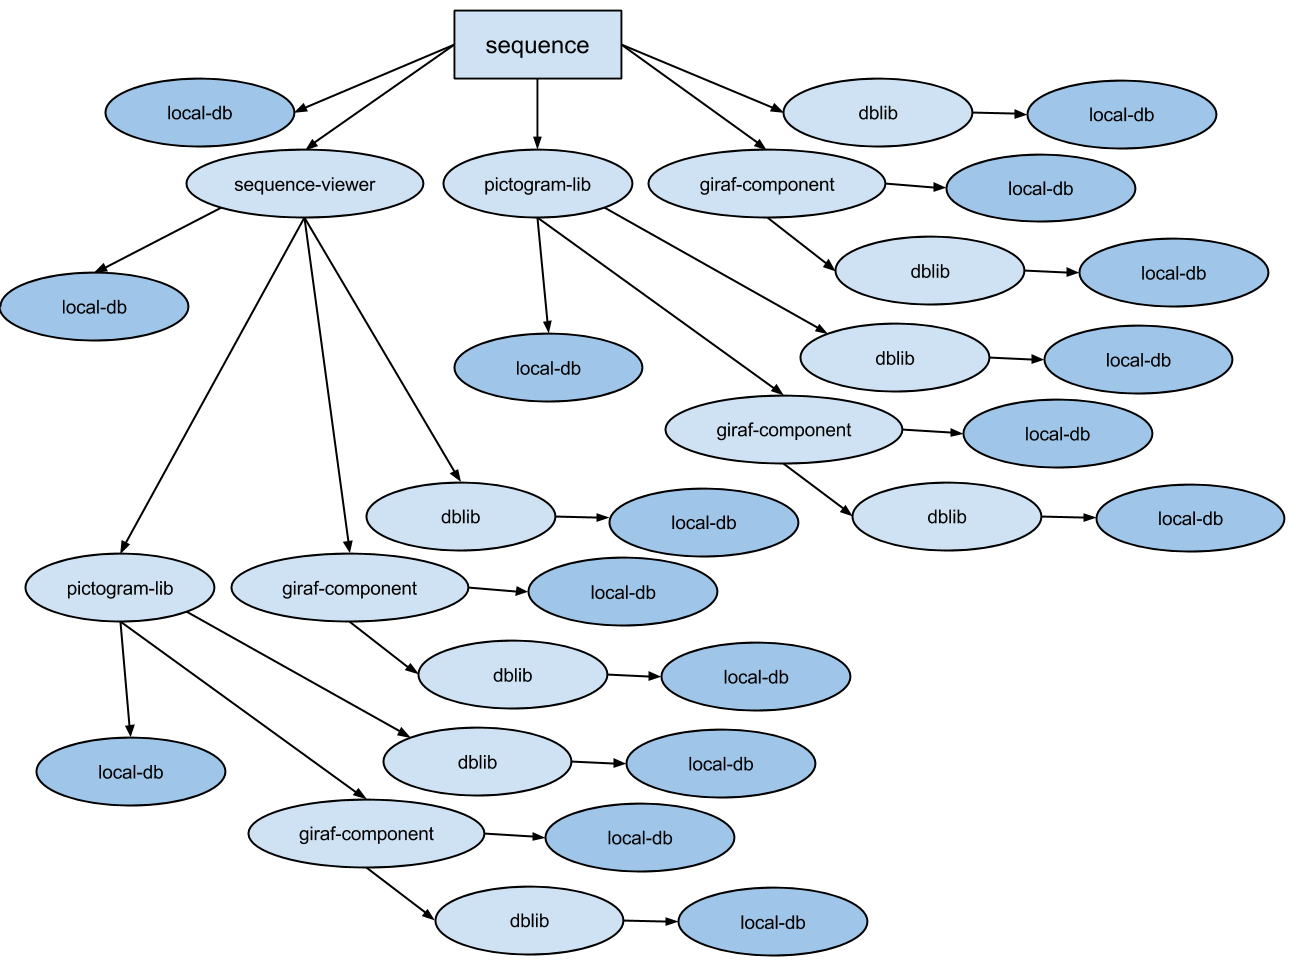
\includegraphics[width= 0.8 \textwidth]{pictures/oldbuild.png}
	\end{figure}
\end{frame}
\begin{frame}
	\frametitle{Metadata}
		\begin{itemize}
			\item Recursively
			\item Manuel Copy paste
			\item Library (.jar)			
		\end{itemize}
\end{frame}
\begin{frame}
	\frametitle{Squenceviewer \& Pictosearch}
	\begin{figure}[H]
				\centering
				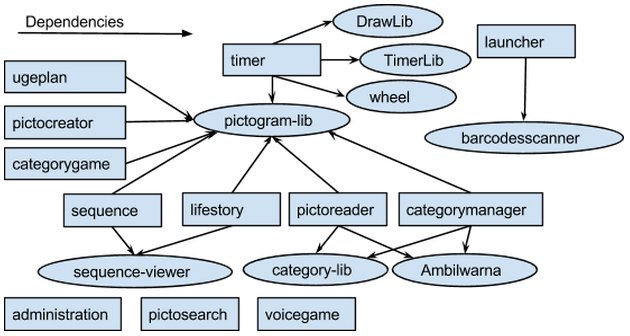
\includegraphics[width= 0.8 \textwidth]{pictures/AppLibependencies.png}
	\end{figure}
\end{frame}
\subsection{Solution}
\begin{frame}
	\frametitle{Libraries}
	\begin{figure}[H]
			\centering
			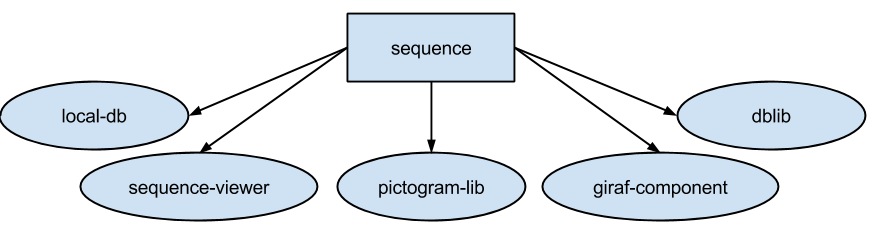
\includegraphics[width= 0.8 \textwidth]{pictures/newbuild.png}
	\end{figure}
\end{frame}
\begin{frame}
	\frametitle{Version control}
	$compile project(':local-db')$
	
	$compile(group: 'dk.aau.cs.giraf', name: 'localDb', version: '5.1.4', ext: 'aar')$
\end{frame}
\begin{frame}
	\frametitle{Remove App dependencies}
	\begin{itemize}
		\item Make Apps into libraries
		\item Standalone			
	\end{itemize}
\end{frame}
\subsection{Change}
\begin{frame}
	\frametitle{Old buildstructure}
	\begin{figure}[H]
			\centering
			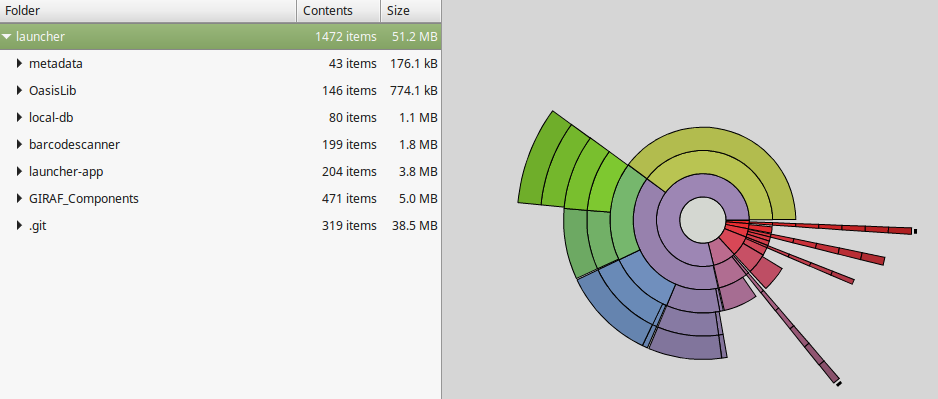
\includegraphics[width= 0.8 \textwidth]{pictures/StatsOld.png}
	\end{figure}
\end{frame}
\begin{frame}
	\frametitle{New buildstructure}
	\begin{figure}[H]
				\centering
				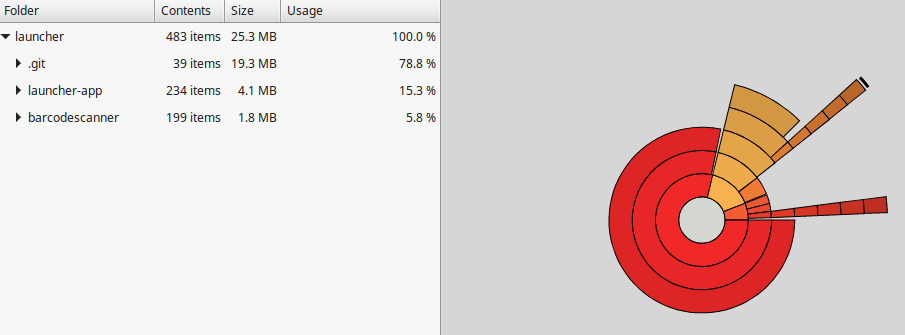
\includegraphics[width= 0.8 \textwidth]{pictures/StatsNew.png}
	\end{figure}
\end{frame}
\begin{frame}
	\frametitle{stats}
	\begin{itemize}
		\item Size went from 51.2 MB  to 25.3 MB 
		\item Contents went from 1472 items to 	483	items
		\item Buildtime went from \~30 min to \~10 min.	
	\end{itemize}
	Note: more functions in the new.
\end{frame}


